\documentclass[aspectratio=169]{beamer}
%
% Choose how your presentation looks.
%
% For more themes, color themes and font themes, see:
% http://deic.uab.es/~iblanes/beamer_gallery/index_by_theme.html
%
\mode<presentation>
{
  \usetheme{metropolis}      % or try Darmstadt, Madrid, Warsaw, ...
  \usecolortheme{default} % or try albatross, beaver, crane, ...
  \usefonttheme{structurebold}  % or try serif, structurebold, ...
  \setbeamercolor{background canvas}{bg=white}
  \setbeamertemplate{navigation symbols}{}
  \setbeamertemplate{bibliography item}{\insertbiblabel}
  %\setbeamertemplate{caption}[numbered]
} 
\usepackage[english]{babel}
\usepackage[utf8x]{inputenc}
\usepackage{listings}             % Include the listings-package
\hypersetup{
    colorlinks = true,
    linkcolor = {black},
    urlcolor = {blue}
}

\DeclareMathOperator*{\argmin}{arg\,min}

\title[Deep Learning and Temporal Data Processing]{Deep Learning and Temporal Data Processing}
\subtitle{1 - Deep Neural Networks}
\institute{University of Modena and Reggio Emilia}
\author{Andrea Palazzi}
\date{June 21th, 2017}

\def\thisframelogos{}

\newcommand{\framelogo}[1]{\def\thisframelogos{#1}}
\newcommand{\R}{\mathbb{R}}

\addtobeamertemplate{frametitle}{}{%
\begin{tikzpicture}[remember picture,overlay]
\node[anchor=north east] at (current page.north east) {%
    \foreach \img in \thisframelogos {%
        %\hspace{.5ex}%
        \includegraphics[height=3.5ex]{\img}%
    }%
};
\end{tikzpicture}}

\begin{document}

\framelogo{logo_unimore_white.png}

\bgroup
\renewcommand{\insertframenumber}{}
\begin{frame}[noframenumbering]
  \titlepage
\end{frame}
\egroup
\begin{frame}{Agenda}
  \tableofcontents
\end{frame}


%%%%%%%%%%%%%%%%%%%%%%%%%%%%%%%%%%%%%%%%%%%%%%%%%%%%%%%%%%%%%%%%%%
%%%%%%%%%%%%%%%%%%%%%%%%%%%%%%%%%%%%%%%%%%%%%%%%%%%%%%%%%%%%%%%%%%
%%%%%%%%%%%%%%%%%%%%%%%%%%%%%%%%%%%%%%%%%%%%%%%%%%%%%%%%%%%%%%%%%%

\section{Introduction}

%%%%%%%%%%%%%%%%%%%%%%%%%%%%%%%%%%%%%%%%%%%%%%%%%%%%%%%%%%%%%%%%%%

\begin{frame}{Deep Neural Networks: overview}
\cite{yu2015multi}
\end{frame}

%%%%%%%%%%%%%%%%%%%%%%%%%%%%%%%%%%%%%%%%%%%%%%%%%%%%%%%%%%%%%%%%%%
%%%%%%%%%%%%%%%%%%%%%%%%%%%%%%%%%%%%%%%%%%%%%%%%%%%%%%%%%%%%%%%%%%
%%%%%%%%%%%%%%%%%%%%%%%%%%%%%%%%%%%%%%%%%%%%%%%%%%%%%%%%%%%%%%%%%%

\section{Linear classifiers}

\begin{frame}{Linear Classifier}
For the purpose of this lecture, we'll stick to the task of image classification.\\
Let's assume we have a training dataset of $N$ images
\begin{equation*}
x_i \in \R^D, i = 1, \dots, N
\end{equation*}
that we want to classify into $K$ distinct classes.\\
Thus, training set is made by couples:
\begin{equation*}
(x_i, y_i),\ where \, y_i \in \{1, \dots, K\}
\end{equation*}
Our goal is to define a function $f: \R^D \mapsto \R^K$ that maps images to class scores.
\end{frame}

%%%%%%%%%%%%%%%%%%%%%%%%%%%%%%%%%%%%%%%%%%%%%%%%%%%%%%%%%%%%%%%%%%

\begin{frame}{Linear Classifier}
Making a real-world example: let's take the \texttt{CIFAR-10} dataset, which consists of $N=60000$ 32x32 RGB images belonging to 10 different classes.\\
\begin{figure}
\begin{tabular}{c}
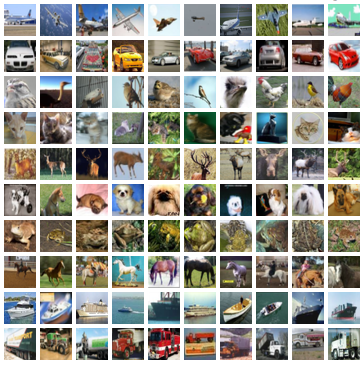
\includegraphics[width=0.4\textwidth]{img/dnn/cifar10.png}
\end{tabular}
\end{figure}
\end{frame}

%%%%%%%%%%%%%%%%%%%%%%%%%%%%%%%%%%%%%%%%%%%%%%%%%%%%%%%%%%%%%%%%%%

\begin{frame}{Linear Classifier}
Each image is $32$x$32$x$3$, thus it can be thought as a column vector $x_i \in \R^{3072}$.\\
Now we can define a \textbf{linear mapping}:
\begin{equation*}
f(x_i,W,b) = Wx_i + b
\end{equation*}
where the parameters are:
\begin{itemize}
\item the weight matrix $W \in \R^{10 x 3072}$ 
\item the bias vector $b \in \R^{10}$.
\end{itemize}
\small{Intuitively, our goal is to learn the parameters from the training set \emph{s.t.} when a new test image $x^{test}_i$ is given as input, the score of the correct class is higher that the scores of other classes.}
\end{frame}

%%%%%%%%%%%%%%%%%%%%%%%%%%%%%%%%%%%%%%%%%%%%%%%%%%%%%%%%%%%%%%%%%%\\

\begin{frame}{Linear Classifier}
\begin{figure}
\begin{tabular}{c}
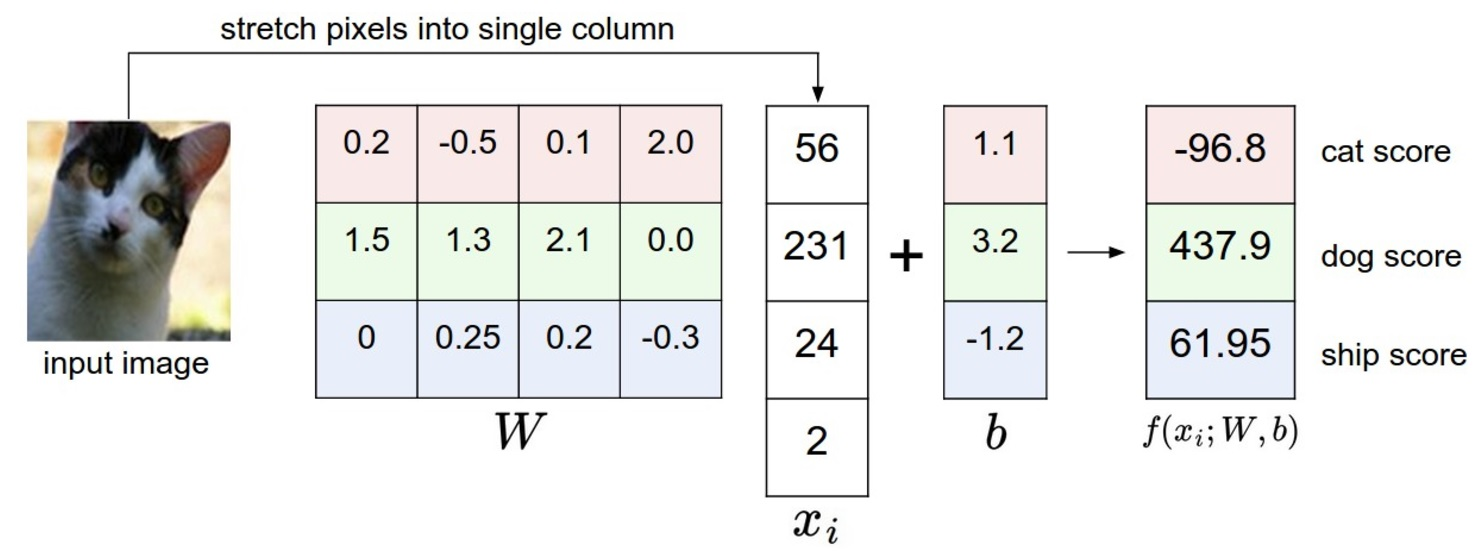
\includegraphics[width=0.8\textwidth]{img/dnn/linear_classifier.jpg}
\end{tabular}
\end{figure}
\small{Example of mapping an image to a score. For the sake of visualization, here the image is assumed to have only 4 grayscale pixels.}
\end{frame}

%%%%%%%%%%%%%%%%%%%%%%%%%%%%%%%%%%%%%%%%%%%%%%%%%%%%%%%%%%%%%%%%%%\\

\begin{frame}{Logistic Regression}

\end{frame}

%%%%%%%%%%%%%%%%%%%%%%%%%%%%%%%%%%%%%%%%%%%%%%%%%%%%%%%%%%%%%%%%%%\\

\begin{frame}{Softmax Classifier}
First let's introduce the \textbf{softmax function}:
\begin{equation*}
softmax_j(\textbf{z}) = \frac{e^{z_j}}{\sum_k e^{z_k}}
\end{equation*}
It takes a vector of arbitrary real-valued scores $\textbf{z}$ and squashes it to a vector of values between zero and one that sum to one.\\
\emph{e.g.}
\begin{equation*}
\textbf{z} = \begin{bmatrix}1.2\\5.1\\2.7\end{bmatrix}
\quad softmax(\textbf{z}) = \begin{bmatrix}0.018\\0.90\\0.08\end{bmatrix}
\end{equation*}
\end{frame}

%%%%%%%%%%%%%%%%%%%%%%%%%%%%%%%%%%%%%%%%%%%%%%%%%%%%%%%%%%%%%%%%%%\\

\begin{frame}{Softmax Classifier}
\textbf{Softmax Classifier} generalizes Logistic Regression classifier to multi-class classification.\\
\vspace{0.2cm}
In the Softmax classifier the scores of linear function mapping $f(x_i,W) = Wx_i$ are interpreted as unnormalized log probabilities and we use the \textbf{cross-entropy loss}:
\begin{equation*}
L_i = -log\left(\frac{e^{f_{y_{i}}}}{\sum_j e^{f_{j}}}\right)
\end{equation*}
\small{Prove yourself that this loss function makes sense.}
%Softmax Classifier has the appealing property to produce an easy-to-interpret output, that is the normalized score confidence for each class.

\end{frame}

%%%%%%%%%%%%%%%%%%%%%%%%%%%%%%%%%%%%%%%%%%%%%%%%%%%%%%%%%%%%%%%%%%
%%%%%%%%%%%%%%%%%%%%%%%%%%%%%%%%%%%%%%%%%%%%%%%%%%%%%%%%%%%%%%%%%%
%%%%%%%%%%%%%%%%%%%%%%%%%%%%%%%%%%%%%%%%%%%%%%%%%%%%%%%%%%%%%%%%%%

\section{Neural Networks}

\begin{frame}{Introduction}
Neural Networks are a mathematical model \textbf{coarsely} inspired by the way our own brain works.
\begin{figure}
\begin{tabular}{c}
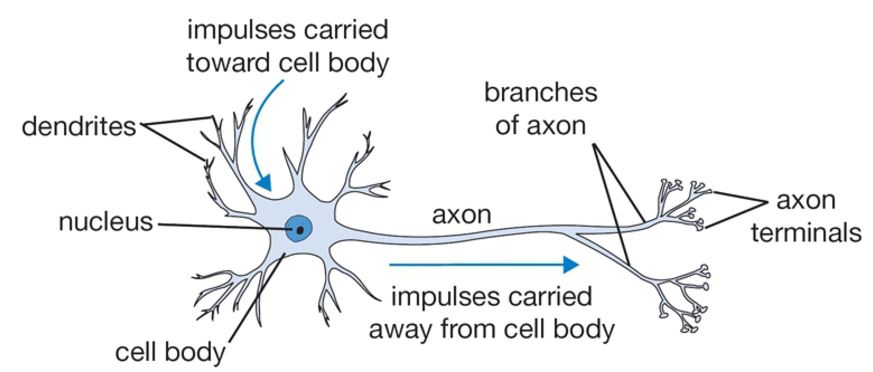
\includegraphics[width=0.4\textwidth]{img/dnn/biological_neuron.jpg}
\end{tabular}
\end{figure}
\small{Neurons are the basic computational unit of our brain. Approximately 86 billion neurons can be found in the human nervous system and they are connected with approximately $10^{14}$ - $10^{15}$ \textbf{synapses}. Each neuron receives input signals from its \textbf{dendrites} and produces output signals along its (single) \textbf{axon}. The axon eventually branches out and connects via synapses to dendrites of other neurons.}
\end{frame}

%%%%%%%%%%%%%%%%%%%%%%%%%%%%%%%%%%%%%%%%%%%%%%%%%%%%%%%%%%%%%%%%%%

\begin{frame}{Modeling a Single Neuron}
More formally, we can model a single \textbf{neuron} as follows:
\begin{figure}
\begin{tabular}{c}
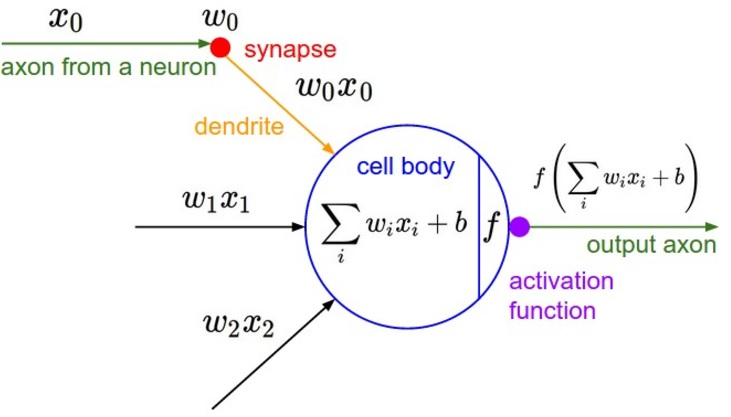
\includegraphics[width=0.4\textwidth]{img/dnn/single_neuron.jpg}
\end{tabular}
\end{figure}
Each neuron can have multiple inputs. The neuron's output is the dot product between the inputs and its weights, plus the bias: then, a non-linearity is applied.
\end{frame}

%%%%%%%%%%%%%%%%%%%%%%%%%%%%%%%%%%%%%%%%%%%%%%%%%%%%%%%%%%%%%%%%%%

\begin{frame}{Modeling a Single Neuron}
It's easy to see that a single neuron can be used to implement a binary classifier.\\
\vspace{1cm}
Indeed, when \textbf{cross-entropy loss} is applied to neuron's output, we can optimize a \textbf{binary Softmax classifier} (\emph{a.k.a.} Logistic regression).
\end{frame}


%%%%%%%%%%%%%%%%%%%%%%%%%%%%%%%%%%%%%%%%%%%%%%%%%%%%%%%%%%%%%%%%%%\\

\begin{frame}{Neural Networks}
When we connect an ensemble of neurons in an acyclic graph is when the magic happens and we get an actual \textbf{neural network}.
\vspace{0.5cm}
\begin{columns}
\begin{column}{0.48\textwidth}
\centering
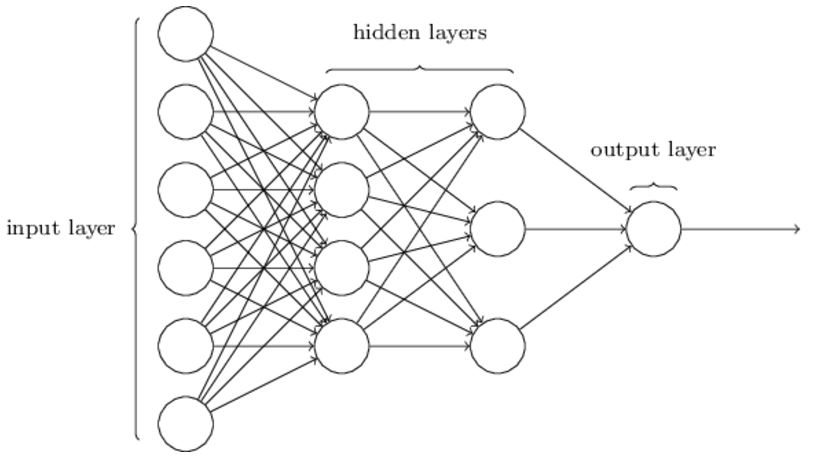
\includegraphics[width=1.0\textwidth]{img/dnn/neural_network.jpg}    \end{column}
\begin{column}{0.48\textwidth}
Neural networks are arranged in \textbf{layers}, with one \textit{input layer}, one \textit{output layer} and $N$ \textit{hidden layers} in the middle.\\
\vspace{0.5cm}
\textit{\small{The network depicted here has a total of $47$ learnable parameters. Does this make sense to you?}}
\end{column}
\end{columns}
\end{frame}

%%%%%%%%%%%%%%%%%%%%%%%%%%%%%%%%%%%%%%%%%%%%%%%%%%%%%%%%%%%%%%%%%%

\begin{frame}{Neural Networks}
From the computational point of view, we can express the 4-layer network previously depicted as follows.
\begin{equation*}
a
\end{equation*}

\end{frame}

%%%%%%%%%%%%%%%%%%%%%%%%%%%%%%%%%%%%%%%%%%%%%%%%%%%%%%%%%%%%%%%%%%

\begin{frame}{Deep Neural Networks: why now}
\end{frame}

%%%%%%%%%%%%%%%%%%%%%%%%%%%%%%%%%%%%%%%%%%%%%%%%%%%%%%%%%%%%%%%%%%
%%%%%%%%%%%%%%%%%%%%%%%%%%%%%%%%%%%%%%%%%%%%%%%%%%%%%%%%%%%%%%%%%%
%%%%%%%%%%%%%%%%%%%%%%%%%%%%%%%%%%%%%%%%%%%%%%%%%%%%%%%%%%%%%%%%%%

\section{Training a DNN}

\begin{frame}{Forward propagation}

Forward propagation is the process of computing the network output given its input.

\end{frame}

\begin{frame}{Backpropagation}

\end{frame}

%%%%%%%%%%%%%%%%%%%%%%%%%%%%%%%%%%%%%%%%%%%%%%%%%%%%%%%%%%%%%%%%%%
%%%%%%%%%%%%%%%%%%%%%%%%%%%%%%%%%%%%%%%%%%%%%%%%%%%%%%%%%%%%%%%%%%
%%%%%%%%%%%%%%%%%%%%%%%%%%%%%%%%%%%%%%%%%%%%%%%%%%%%%%%%%%%%%%%%%%

\section{Credits}
\begin{frame}{Credits}
These slides heavily borrow from the following Stanford course:
\begin{itemize}
\item \url{http://cs231n.stanford.edu/}
\end{itemize}
if you want to deepen your knowledge of these concepts, I'd really suggest to start from here!\\
\vspace{0.2cm}
Also, nice convolution animations are taken from here:
\begin{itemize}
\item \url{https://github.com/vdumoulin/conv_arithmetic}
\end{itemize}
\end{frame}

%%%%%%%%%%%%%%%%%%%%%%%%%%%%%%%%%%%%%%%%%%%%%%%%%%%%%%%%%%%%%%%%%%
%%%%%%%%%%%%%%%%%%%%%%%%%%%%%%%%%%%%%%%%%%%%%%%%%%%%%%%%%%%%%%%%%%
%%%%%%%%%%%%%%%%%%%%%%%%%%%%%%%%%%%%%%%%%%%%%%%%%%%%%%%%%%%%%%%%%%

\section{References}

\begin{frame}[t]
\frametitle{References}
\bibliographystyle{abbrv}
\bibliography{bibliography}
\end{frame}
\end{document}